\documentclass{report}
\usepackage[margin=1in]{geometry}
\usepackage[T1]{fontenc} % Fontes T1
\usepackage[utf8]{inputenc} % Input UTF8
%\usepackage[backend=biber, style=ieee]{biblatex} % para usar bibliografia
\usepackage{csquotes}
\usepackage[portuguese]{babel} %Usar língua portuguesa
\usepackage{blindtext} % Gerar texto automaticamente
\usepackage[printonlyused]{acronym}
\usepackage{hyperref} % para autoref
\usepackage{graphicx}
\usepackage{subcaption}
\usepackage{float}

\graphicspath{{./imagens/}}

%% TODO -> Reler o Relatório Todo
\begin{document}
	\begin{titlepage}
    	\begin{center}
    		
\includegraphics[width=0.6\textwidth]{logo-isec}
    		
    		\vspace*{\fill}
    		
    		\Huge
    		\textbf{Relatório - Balanceamento de carga em Servidores Web com HAProxy e Keepalived}
    		
    		\huge
    		Disponibilidade e Desempenho
    		
    		\vspace{0.5cm}
    		\LARGE
    		2021 - 2022
    		
    		\vspace{1.5cm}
    		
    		\textbf{Bruno Teixeira}\\
                a2019100036@isec.pt
    		
    		\vfill
    		\vspace*{\fill}
    		
    		\normalsize
    		Licenciatura de Engenharia Informática \\
    		21 de janeiro de 2021
    	\end{center}
    \end{titlepage}

\pagenumbering{roman}


\tableofcontents
% \listoftables     % descomentar se necessário
\listoffigures    % descomentar se necessário



\clearpage
\pagenumbering{arabic}


\chapter{Introdução}\label{chap.introducao}
\paragraph{}
Este trabalho tem como objetivo estudar o balanceamento de carga e o \emph{failover} em servidores \emph{web} com o HAProxy e o KeepAlived. \\
O principal foco é, criar alguns cenários com possíveis falhas, analisar esses cenários, descobrir os pontos fracos e tentar sempre minimizar o \emph{downtime}.
\paragraph{}
Para alcançar este objetivo foram então criadas algumas experiências de modo a perceber como é possível criar uma infraestrutura segura e com um \emph{downtime} reduzido ou até mesmo nulo aplicando ao mesmo tempo o conceito de balanceamento de carga.
\label{chap.introducao}

\paragraph{}


\chapter{Desenvolvimento}\label{Uma label qualquer}

\section{Descrição das tecnologias usadas}

\section{Flask, MariaDB e Galera Cluster}
\paragraph{}
O Flask é um \emph{micro-framework} do \emph{Python} destinado principalmente para pequenas aplicações com requisitos mais simples. O mesmo funciona bastante bem com bases de dados tendo sido este o escolhido para o desenvolvimento da aplicação \emph{web} para este trabalho.\\
Para que a aplicação fosse \emph{stateful} foi então usada uma base de dados em MariaDB, uma vez que a mesma tem uma comunidade enorme na Internet, tornando-a bastante simples de ser utilizada.

\paragraph{}
O \emph{Galera Cluster} é um \emph{cluster} virtual para MariaDB que permite a replicação entre diferentes bases de dados, mantendo assim uma disponibilidade e desempenho alto uma vez que existe mais do que uma base de dados para responder a diferentes \emph{querys} dos clientes, sendo que todas as mudanças feitas numa base de dados são replicadas para a outra.


\section{HAProxy}
\paragraph{}
O HAProxy é um serviço Linux que garante o balanceamento de carga para HTTP e TCP. Na prática, o mesmo recebe as conexões dos utilizadores e atua como \emph{proxy}, criando um canal de comunicação entre o utilizador e um dos \emph{webservers}.

\paragraph{}
O HAProxy funciona em dois modos diferentes, HTTP ou TCP.

\begin{itemize}
  \item Quando opera em TCP dizemos que é um \emph{Proxy} de camada 4 (OSI)
        \begin{itemize}
          \item Quando o HAProxy opera neste modo, o mesmo apenas tem acesso a qual IP e Porto o cliente está a tentar aceder, não conseguindo assim ver a informação trocada entre de ambas as partes.
        \end{itemize}
  \item Quando opera em HTTP dizemos que é um \emph{Proxy} de camada 7 (OSI)
    \begin{itemize}
      \item Quando o HAProxy opera neste modo, o mesmo tem acesso a toda a informação, logo estamos a confiar no mesmo para ter acesso a esses dados, dados que transitam de um lado para o outro.
        \end{itemize}
\end{itemize}


\section{KeepAlived}
\paragraph{}
O objetivo principal do KeepAlived é fornecer instalações simples para existir balanceamento de carga e alta disponibilidade (a alta disponibilidade é alcançada pelo protocolo VRRP) para sistemas baseados em Linux. O Keepalived agrega então um conjunto de servidores de balanceamento de carga (HAProxy), e consoante a saúde dos mesmos, ele toma decisões sobre pelo qual deverá passar a operacionalização.


\section{Ambiente para as experiências}
\paragraph{}
Para serem feitas algumas experiências foi criado um ambiente com várias máquinas virtuais, estando estas agregadas a um virtualizador ESXi, ou seja, todas as máquinas estão na mesma LAN.

\begin{itemize}
  \item \textbf{webserver01} - 192.168.1.180
  \item \textbf{webserver02} - 192.168.1.181

  \item \textbf{mariadb01} - 192.168.1.182
  \item \textbf{mariadb02} - 192.168.1.186
    
  \item \textbf{haproxy01} - 192.168.1.183
  \item \textbf{haproxy02} - 192.168.1.184
    
  \item \textbf{haproxy03} - 192.168.1.185
  \item \textbf{haproxy04} - 192.168.1.187
\end{itemize}

\subsection{Aplicação Web}
\paragraph{}
Como descrito anteriormente, foi criada uma aplicação em Flask. Esta aplicação funciona como uma espécie de lista de compras em que o utilizador depois de fazer o \emph{login}, consegue adicionar e eliminar produtos do seu cesto.

\begin{figure}[H]
\center
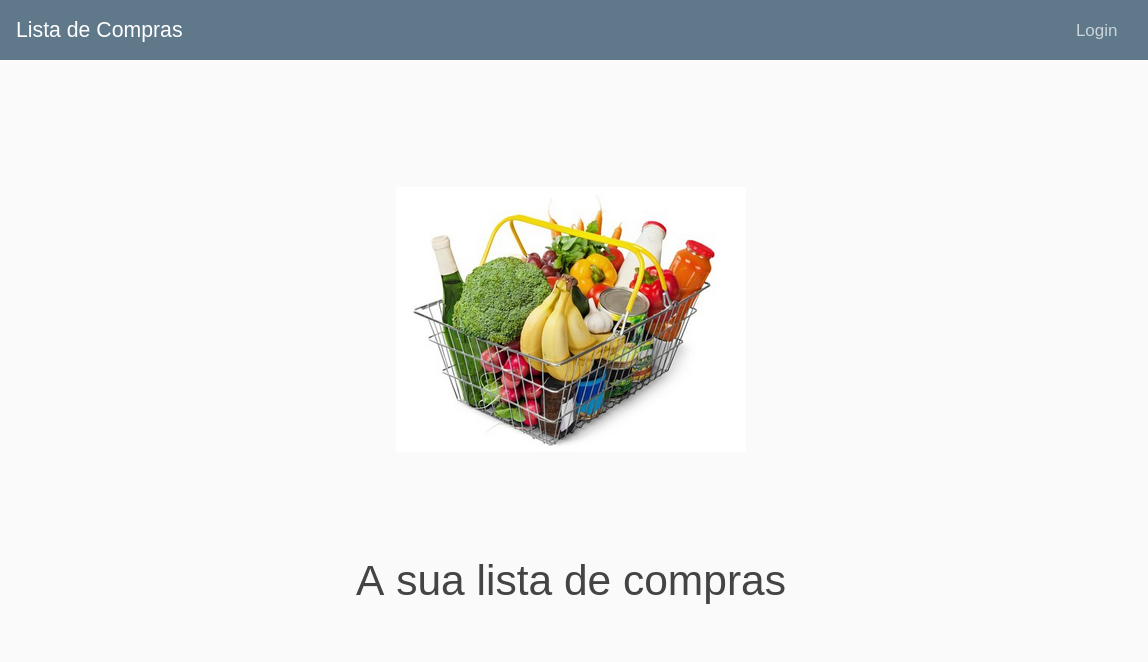
\includegraphics[width=12cm]{imagens/aplicacao_web/index.png}
\caption{Index - Aplicação Web} 
\label{fig.nav}
\end{figure}


\begin{figure}[H]
\center
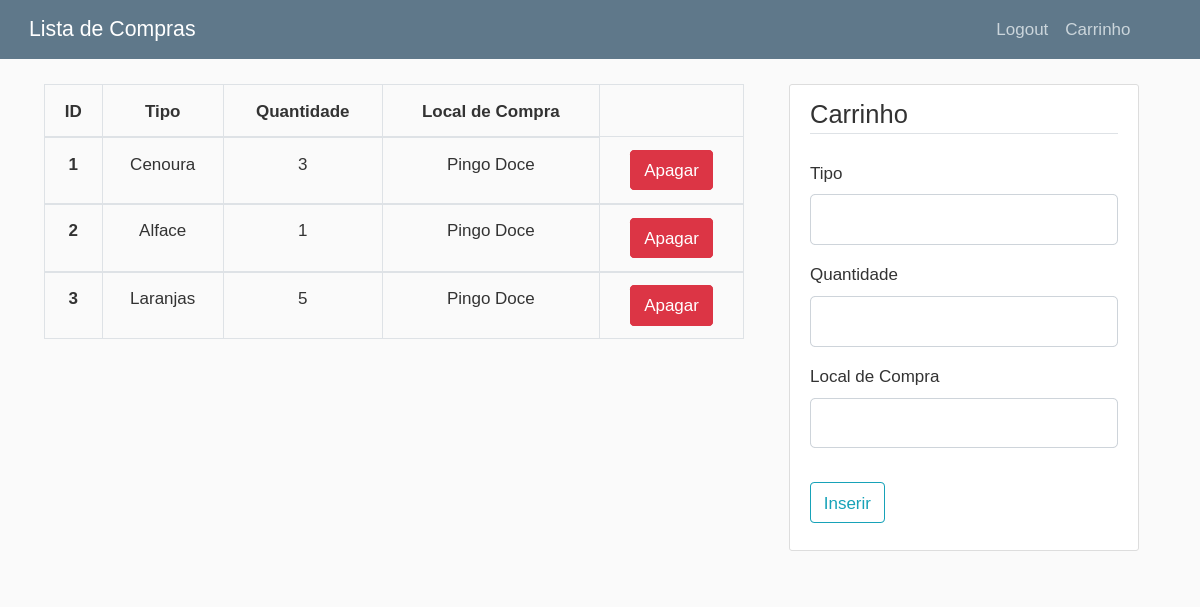
\includegraphics[width=12cm]{imagens/aplicacao_web/carrinho.png}
\caption{Carrinho - Aplicação Web}
\label{fig.nav}
\end{figure}

\subsection{Configuração do HAProxy}
\paragraph{}
No ficheiro de configuração do HAProxy (localizado em \textbf{\emph{/etc/haproxy/haproxy.cfg}}) existem 5 secções, sendo que estas definem como é que o servidor se comporta, quais são as definições por omissão, e como é que o cliente faz pedidos e recebe respostas.
\begin{itemize}
  \item \textbf{global}
    \begin{itemize}
      \item Nesta primeira secção estão definidas as medidas em que o processo vai operar, sendo estas medidas de um nível mais baixo, ou seja, relacionadas com o sistema operativo.
    \end{itemize}
          
  \item \textbf{defaults}
    \begin{itemize}
      \item Esta secção não é obrigatória, no entanto permite reduzir a duplicação de comandos, uma vez que as configurações feitas aqui são aplicadas na secção \textbf{\emph{frontend}} e \textbf{\emph{backend}}.
    \end{itemize}
      
  \item \textbf{listen}
    \begin{itemize}
      \item Aqui podemos combinar o \textbf{frontend} e \textbf{backend} ao mesmo tempo. Isto é útil, pois é aqui feito o redirecionamento para o \textbf{\emph{endpoint}} de estatisticas.
     \end{itemize}
      
   \item \textbf{frontend}
     \begin{itemize}
       \item Nesta secção definimos como é que os pedidos dos utilizadores irão ser encaminhados para o \textbf{backend}.
     \end{itemize}

       
   \item \textbf{backend}
     \begin{itemize}
       \item Aqui definimos os \textbf{\emph{webservers}} que vão operar na infraestrutura, definindo tambem o algoritmo de \textbf{\emph{load balancing}} a ser utilizado
     \end{itemize}
\end{itemize}


\begin{figure}[H]
\center
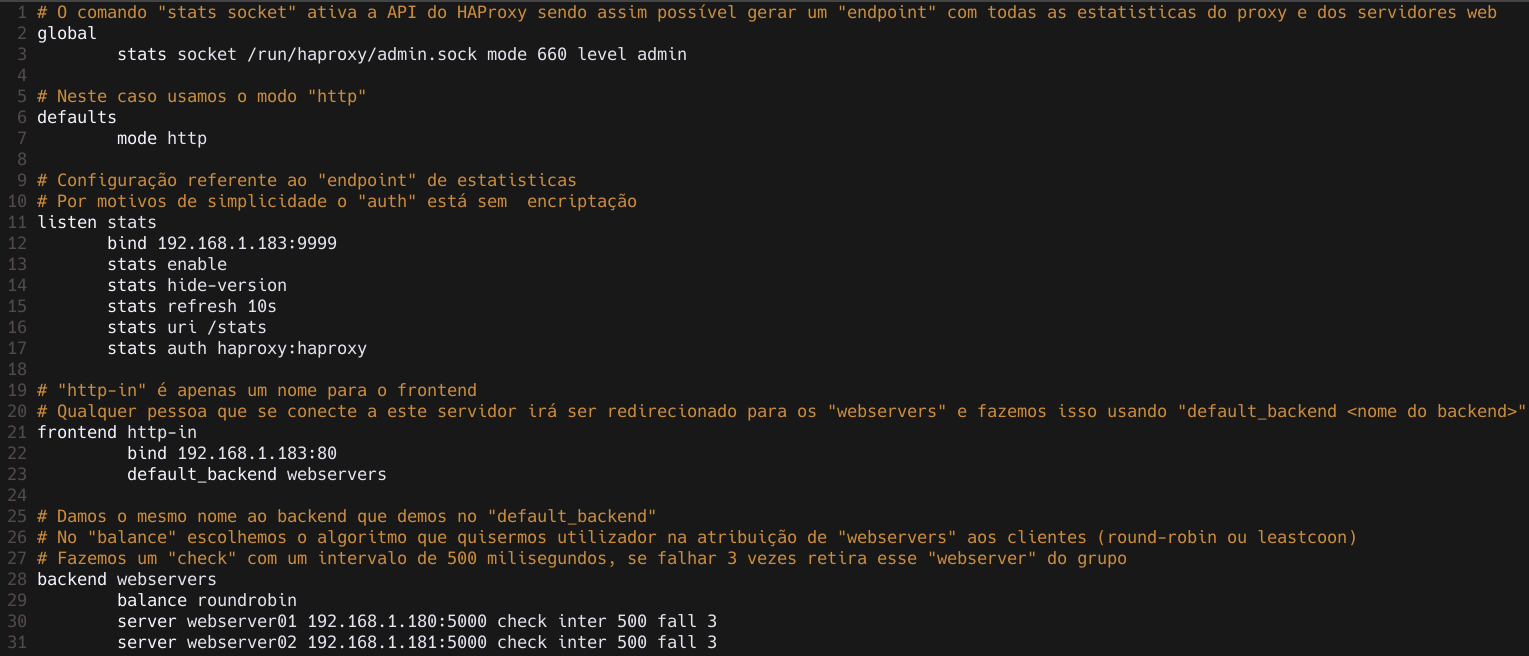
\includegraphics[width=16cm]{imagens/haproxy_config.png}
\caption{Configuração - HAProxy}
\label{fig.nav}
\end{figure}

Conforme foi configurado o HAProxy, ao acedermos a \textbf{\emph{http://192.168.1.183:9999/stats}} conseguimos visualizar uma página \emph{web} com várias estatísticas sobre os \emph{webservers}. 

\begin{figure}[H]
\center
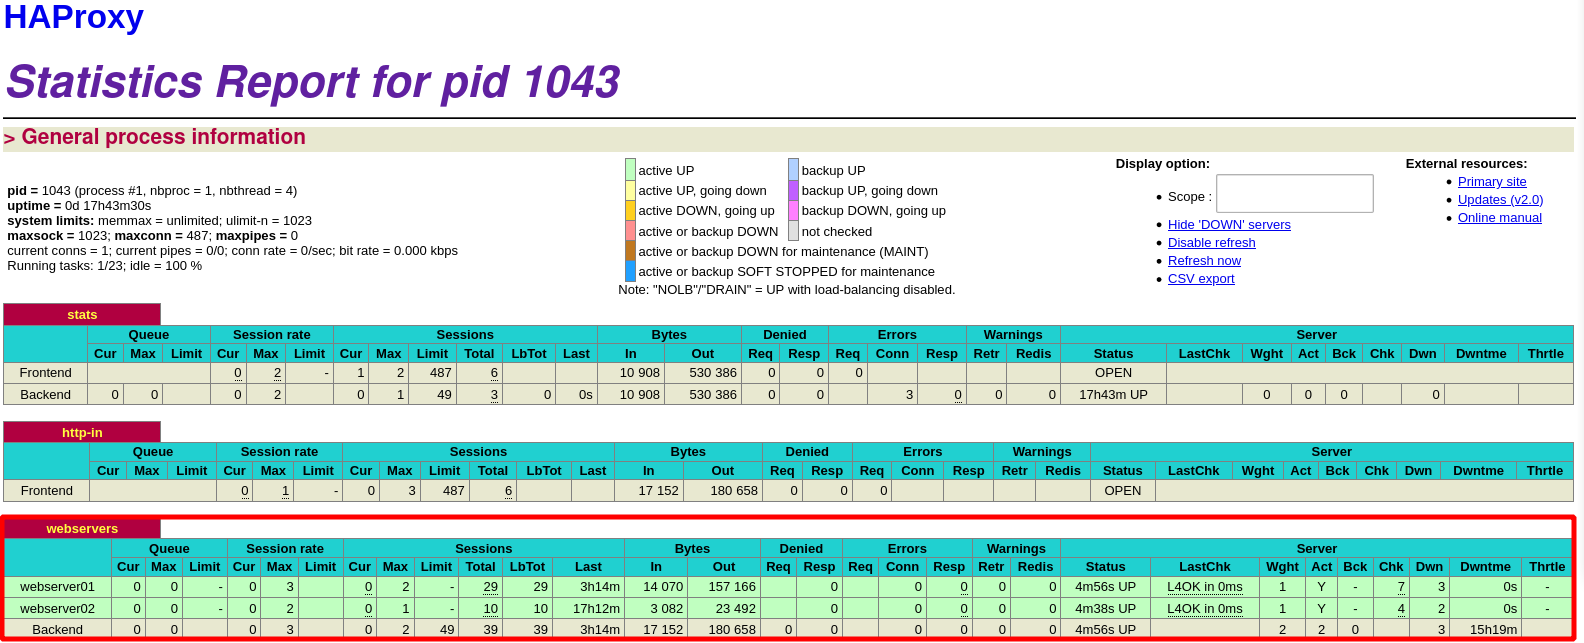
\includegraphics[width=17cm]{imagens/haproxy_stats.png}
\caption{Estatísticas - HAProxy}
\label{fig.nav}
\end{figure}


\subsection{Configuração do KeepAlived}
\paragraph{}
No ficheiro de configuração do Keepalived (localizado em \textbf{\emph{/etc/keepalived/keepalived.conf}}), foi criado um \textbf{vrrp\_script} com o intuito de verificar, com um intervalo de 2 em 2 milisegundos, se o haproxy está a funcionar corretamente. Se o mesmo não estiver a funcionar, o peso dele diminui em 10 reduzindo assim a sua prioridade tornando o BACKUP num MASTER.\\
Depois disto, foi criado um \textbf{vrrp\_instance} que define uma instância individual do protocolo VRRP com alguns atributos.

\begin{figure}[H]
\center
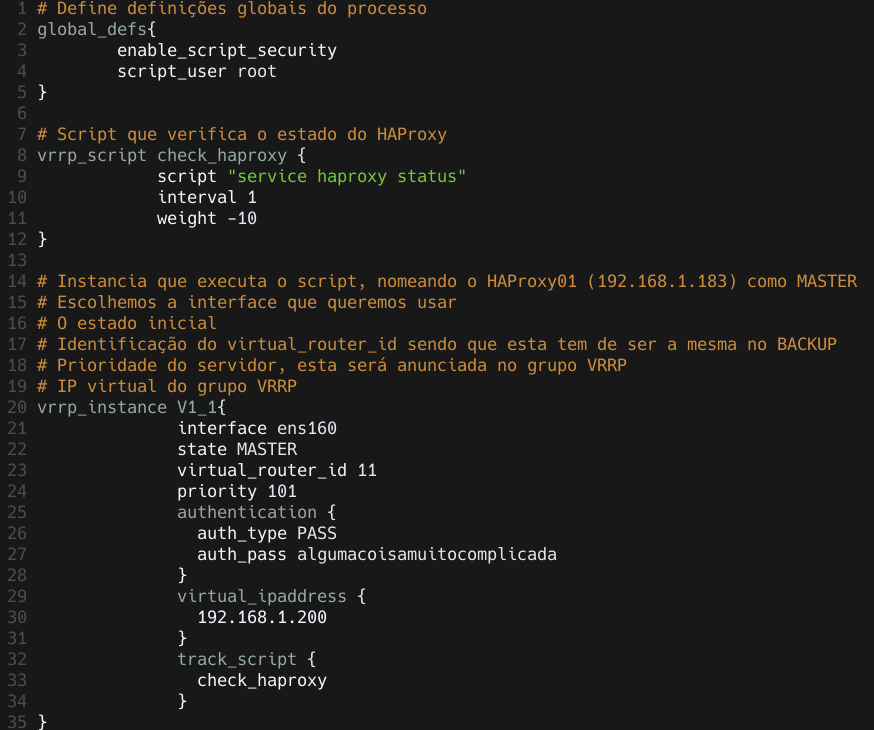
\includegraphics[width=12cm]{imagens/keepalived_config.png}
\caption{Configuração - Keepalived}
\label{fig.nav}
\end{figure}

O mesmo foi feito para o segundo servidor de HAProxy, no entanto foi alterada a prioridade e o estado para definir que este seria o BACKUP.\\

Foi tambem necessário alterar o Ip, para onde faziamos \textbf{\emph{bind}} inicialmente (\textbf{Ip do servidor HAProxy}),  para o novo IP virtual (\textbf{192.168.1.200}) na secção de \textbf{\emph{frontend}} do ficheiro de configuração do HAProxy.

Por fim foi preciso colocar \textbf{\emph{net.ipv4.ip\_nonlocal\_bind=1}} no ficheiro \textbf{\emph{/etc/sysctl.conf}} uma vez que no segundo servidor de HAProxy o IP virtual ainda não está ativo (só fica ativo quando esse for o MASTER), logo não é possível iniciar o \emph{bind}.

\paragraph{}
Esta configuração do KeepAlived apenas foi feita a partir da segunda experiência, uma vez que na primeira ainda não é usado o mesmo para mostrar os riscos que isso tem.

\section{Experiências}

\subsection{Experiência 01}
\paragraph{}
Nesta experiência foi usado um servidor de balanceamento de carga (HAProxy), dois \emph{webservers} e uma base de dados externa (MariaDB). Foi feita uma captura no HAProxy para perceber o que acontecia quando o utilizador fazia um pedido ao mesmo.

\begin{figure}[H]
\center
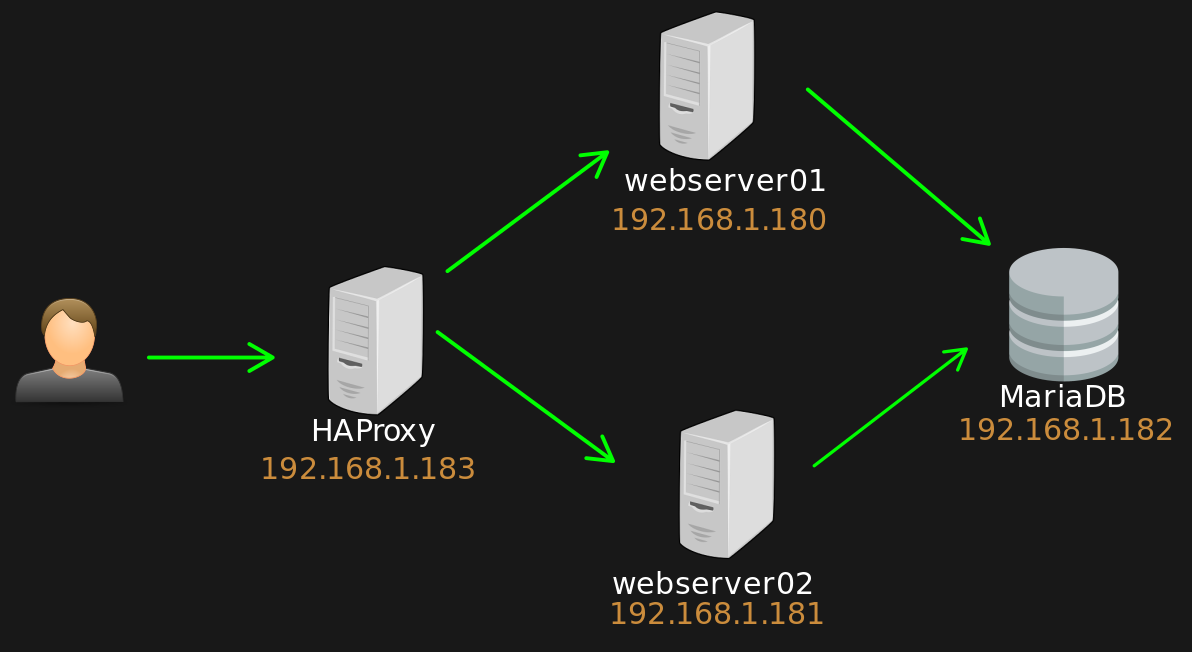
\includegraphics[width=12cm]{imagens/experiencias/01_1.png}
\caption{Esquema - Experiência 01}
\label{fig.nav}
\end{figure}


\subsubsection{Resultado}
Conseguiu-se perceber que o cliente (\textbf{192.168.1.123}) envia um \emph{HTTP GET Request} diretamente ao servidor HAProxy (\textbf{192.168.1.183}).
De seguida, o servidor HAProxy faz um \emph{HTTP GET Request} ao \emph{webserver} disponível, que neste caso foi o \emph{webserver01} (\textbf{192.168.1.180}).
O \emph{webserver01} responde com o \emph{HTTP status code 200}, mostrando que a comunicação ocorreu sem falhas, sendo feito depois um redirecionamento do HAProxy para o cliente.
Imediatamente a seguir foi feito outro pedido pelo mesmo cliente, no entanto consegue-se perceber que, como está a ser usar o algoritmo \textbf{round-robin}, quem respondeu foi o \emph{webserver02}.

\begin{figure}[H]
\center
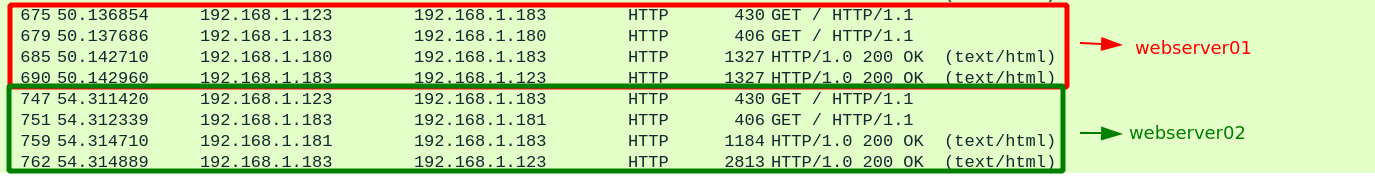
\includegraphics[width=16cm]{imagens/experiencias/01_wireshark.png}
\caption{Wireshark - Experiência 01}
\label{fig.nav}
\end{figure}

\subsubsection{Problemas encontrados na Experiência 01}
\paragraph{}
É percetivel que a experiência feita anteriormente tem alguns problemas, como a existência de dois SPOFs (\textbf{Single Point of Failure}).
\begin{itemize}
  \item Existe um SPOF no HAProxy.
  \item Existe um SPOF na Base de Dados.
\end{itemize}
Ou seja, caso o servidor de HAProxy ou a base de dados deixe de operar, o cliente deixa de ter comunicação com os \emph{webservers}. Sabendo isto continuou-se com mais algumas experiências de modo a resolver estes problemas.

\begin{figure}[H]
\center
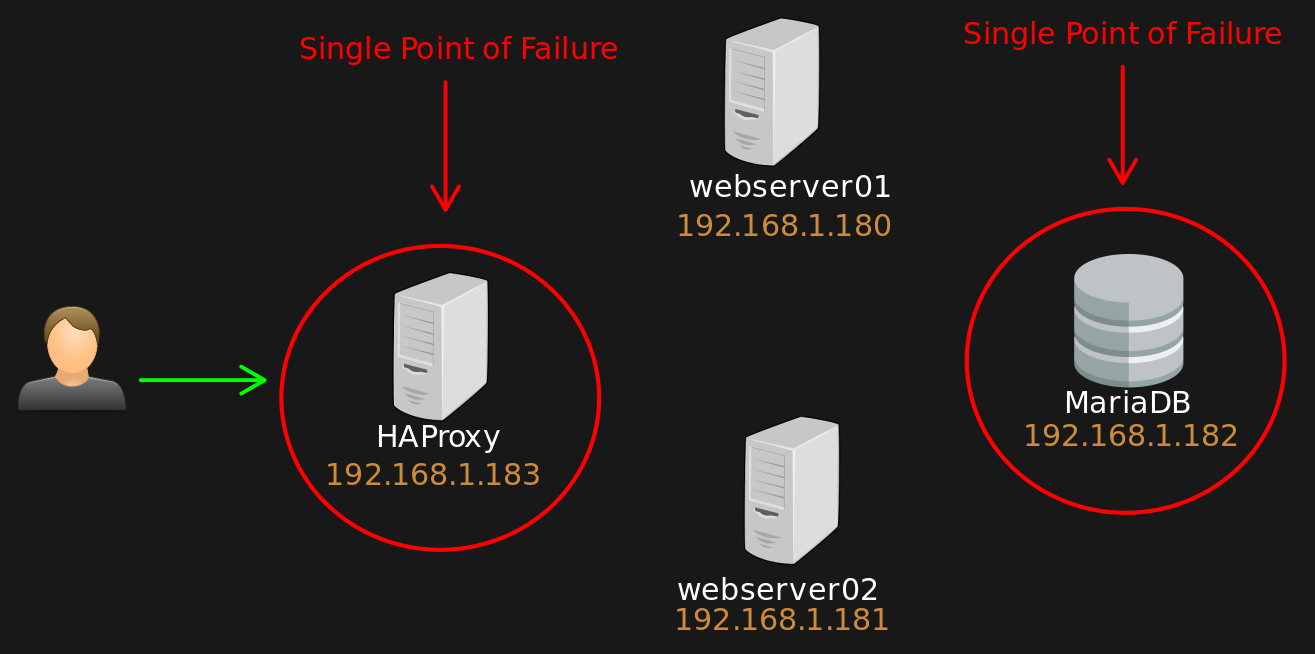
\includegraphics[width=12cm]{imagens/experiencias/01_spof.png}
\caption{Single Point of Failure - Experiência 01}
\label{fig.nav}
\end{figure}


\subsection{Experiência 02}
Nesta segunda experiência apenas foi acrescentado mais um servidor de balanceamento de carga e o serviço de \textbf{KeepAlived} em ambos os servidores de HAProxy.\\
O objetivo da mesma era entender como seria feito o \emph{fail-over} do \textbf{KeepAlived} e o que sucedia depois de um servidor \emph{MASTER} tornar-se \emph{BACKUP} e vice-versa.

\begin{figure}[H]
\center
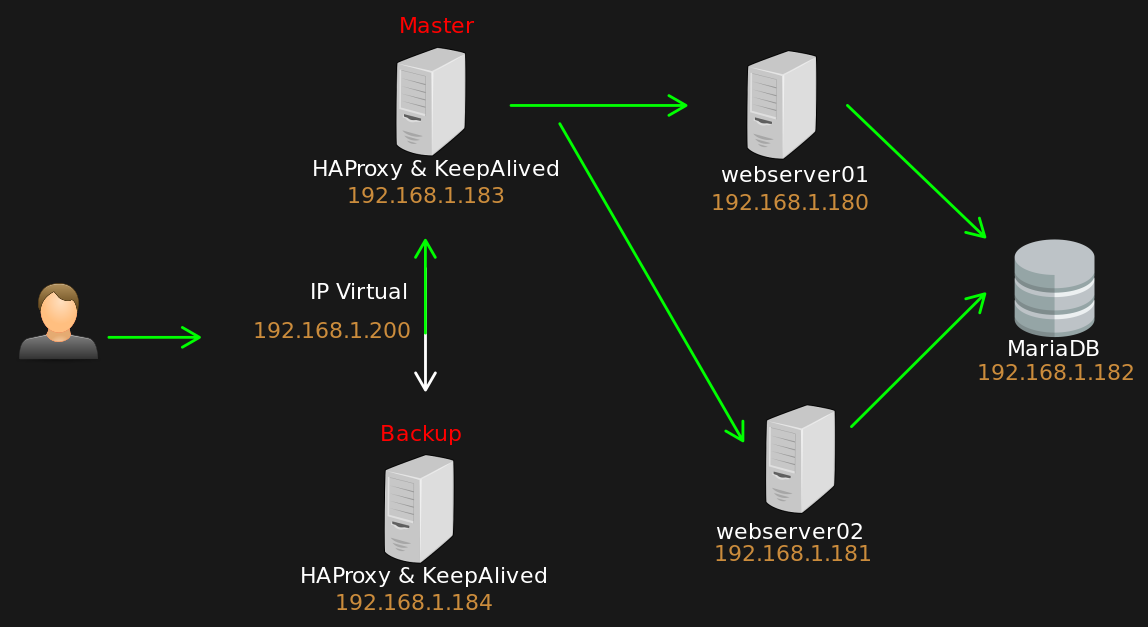
\includegraphics[width=12cm]{imagens/experiencias/02_01.png}
\caption{Esquema - Experiência 02}
\label{fig.nav}
\end{figure}

\begin{figure}[H]
\center
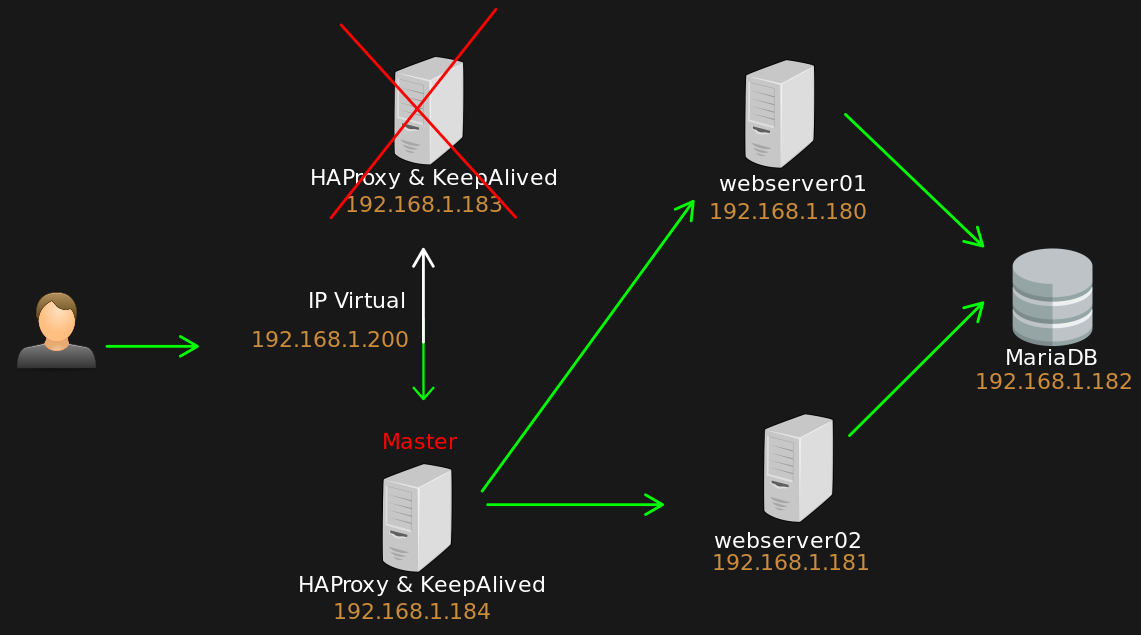
\includegraphics[width=12cm]{imagens/experiencias/02_02.png}
\caption{Esquema com \emph{fail-over} - Experiência 02}
\label{fig.nav}
\end{figure}


\subsubsection{Resultado}
Foram feitas várias capturas, tanto no \textbf{HAProxy01(MASTER)} como no \textbf{HAProxy02(BACKUP)} usando o \emph{wireshark}.\\
Com a captura no \textbf{HAProxy01(192.168.1.183)} percebe-se que o mesmo emite, de segundo em segundo, um \emph{announcement} dizendo a sua prioridade, que neste caso é 101. Isto acontece porque no protocolo VRRP apenas o \emph{MASTER} emite mensagens estando os outros \emph{BACKUPs} à escuta desse aviso.

\begin{figure}[H]
\center
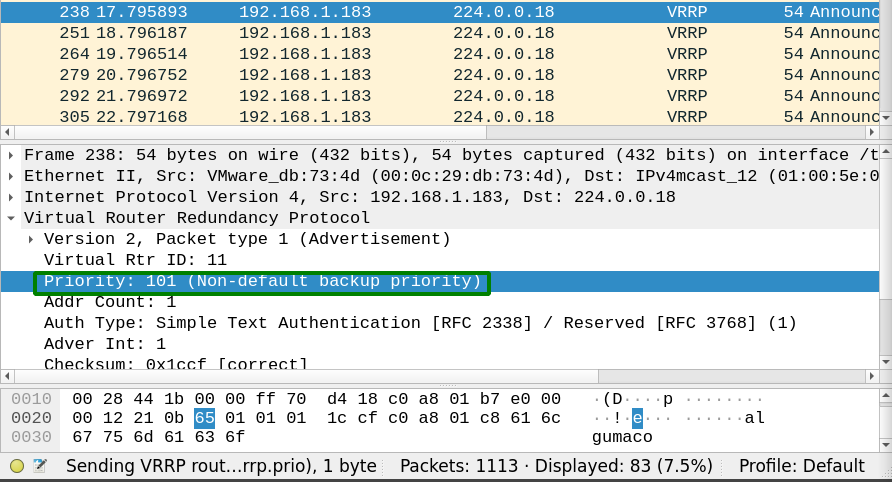
\includegraphics[width=12cm]{imagens/experiencias/02_wireshark.png}
\caption{Wireshark no 192.168.1.183 - Experiência 02}
\label{fig.nav}
\end{figure}

\begin{figure}[H]
\center
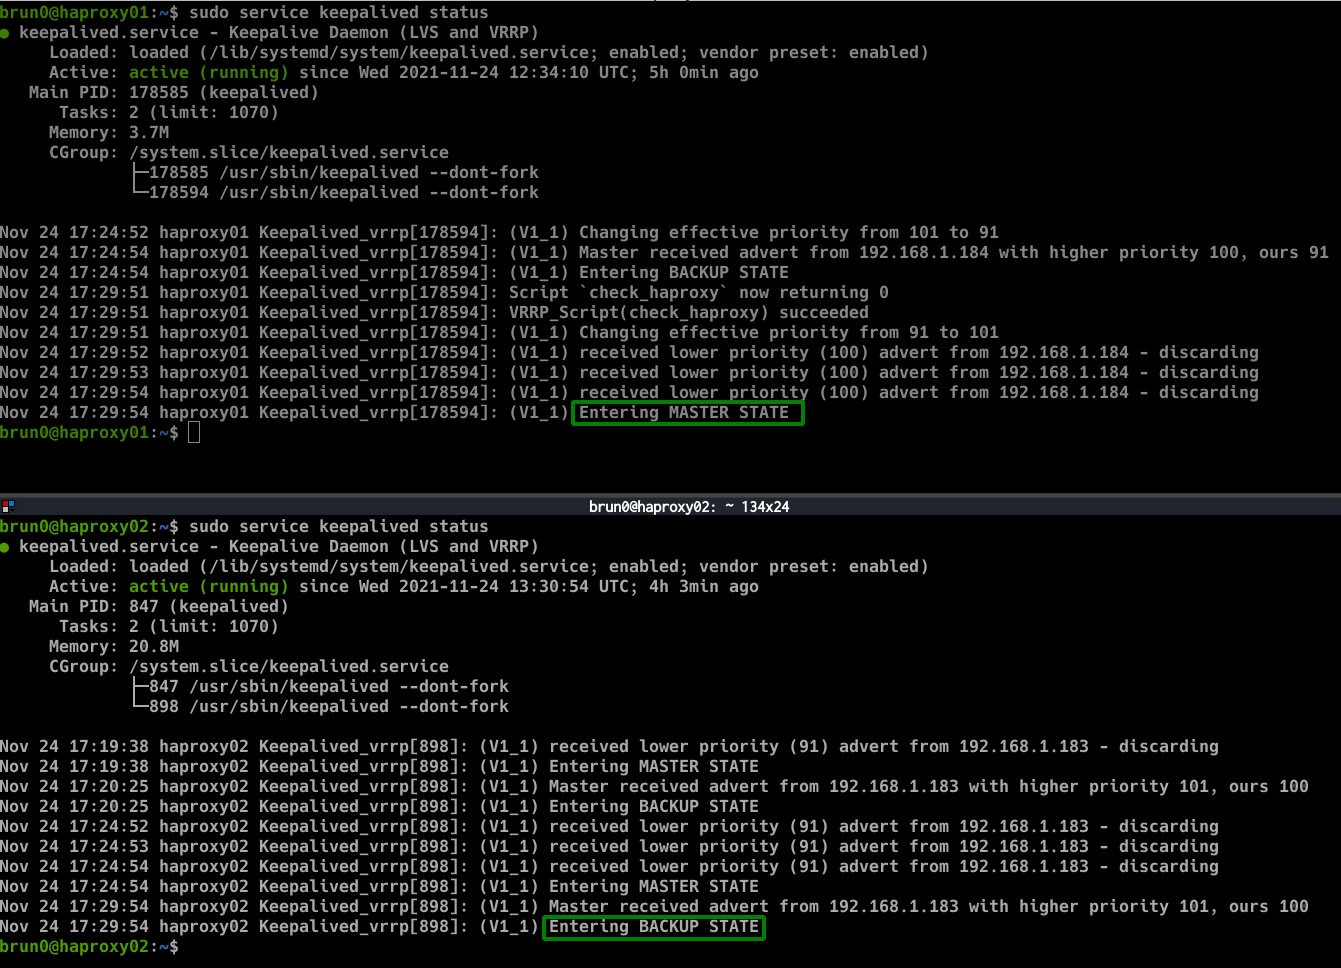
\includegraphics[width=14cm]{imagens/experiencias/02_terminal.png}
\caption{Estado inicial do KeepAlived em ambos os servidores - Experiência 02}
\label{fig.nav}
\end{figure}


\paragraph{}
Depois de desligar o serviço HAProxy do \textbf{HAProxy01(192.168.1.183)}, o mesmo fica com uma prioridade de 91 passando assim para o estado de \emph{BACKUP} ao mesmo tempo que o \textbf{HAProxy02(192.168.1.184)} passa para o estado de \emph{MASTER} uma vez que a sua prioridade é superior (100).

\begin{figure}[H]
\center
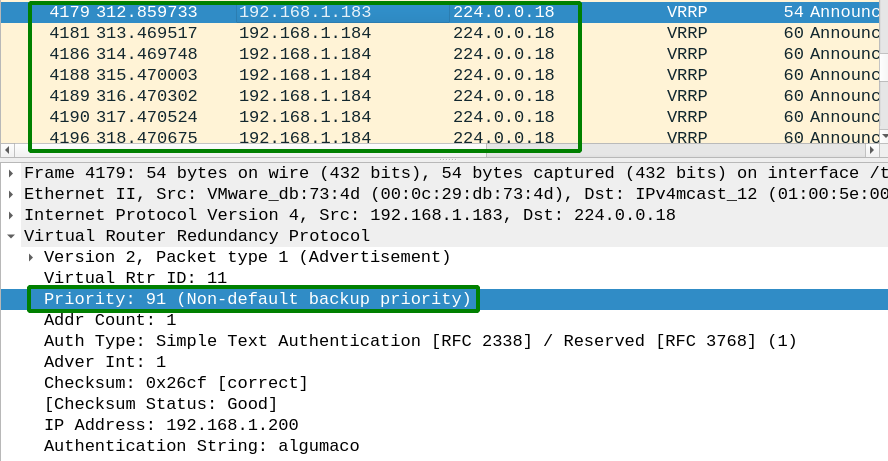
\includegraphics[width=12cm]{imagens/experiencias/02_wireshark_haproxy_desligado.png}
\caption{Wireshark no 192.168.1.183 com o HAProxy desligado - Experiência 02}
\label{fig.nav}
\end{figure}

\begin{figure}[H]
\center
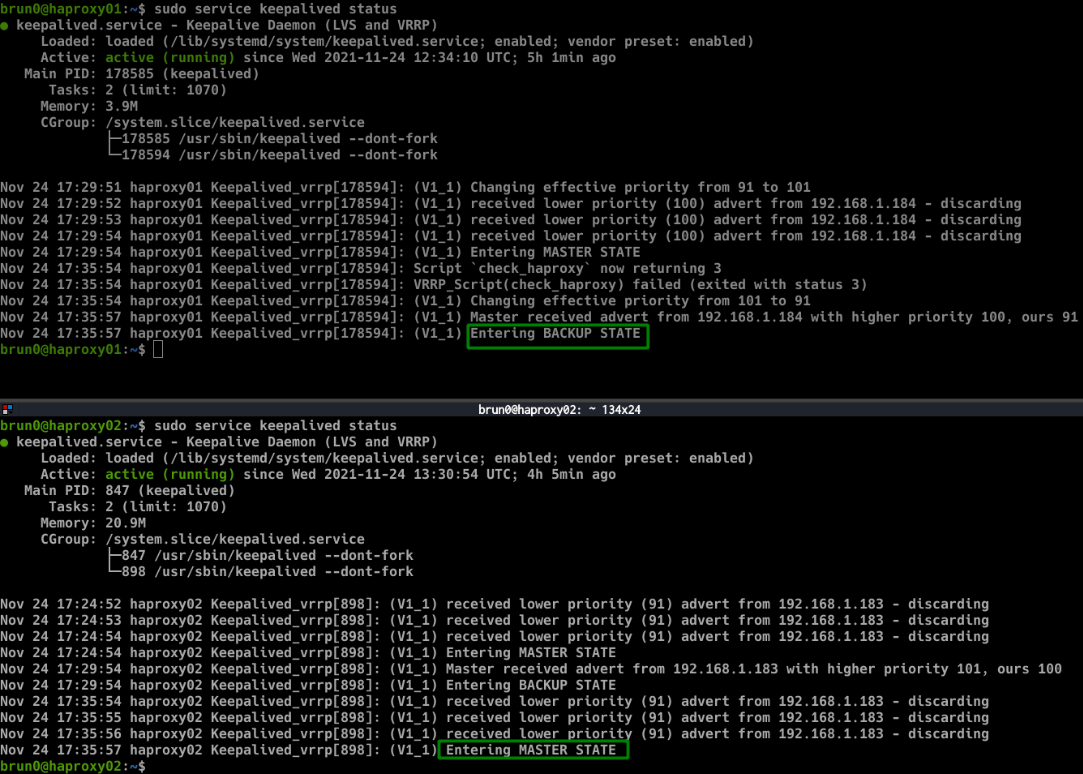
\includegraphics[width=14cm]{imagens/experiencias/02_terminal_haproxy_desligado.png}
\caption{Estado atual do KeepAlived em ambos os servidores - Experiência 02}
\label{fig.nav}
\end{figure}

\paragraph{}
Para terminar, voltou-se a ativar o serviço haproxy no \textbf{HAProxy01(192.168.1.183)} tornando-se assim novamente \emph{MASTER} uma vez que a preempção está ativa por omissão fazendo com que a sua prioridade volte a ser 101 como estava definida inicialmente.

\begin{figure}[H]
\center
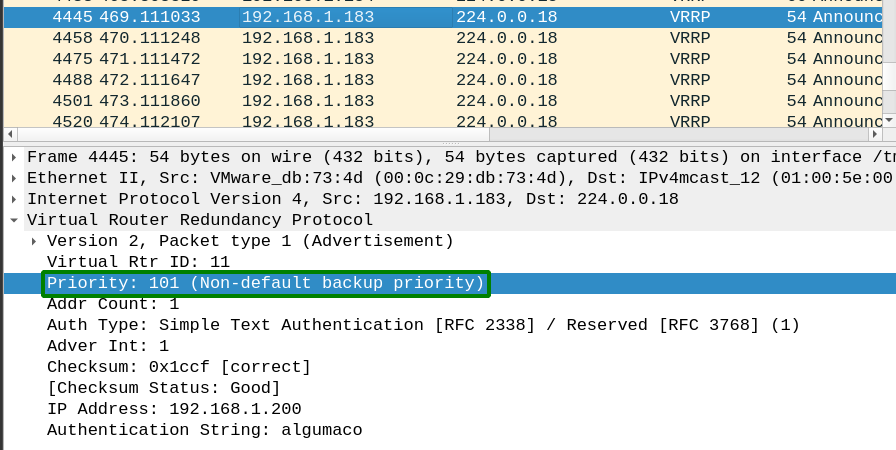
\includegraphics[width=12cm]{imagens/experiencias/02_wireshark_haproxy_retomado.png}
\caption{Wireshark no 192.168.1.183 com o HAProxy retomado - Experiência 02}
\label{fig.nav}
\end{figure}

\begin{figure}[H]
\center
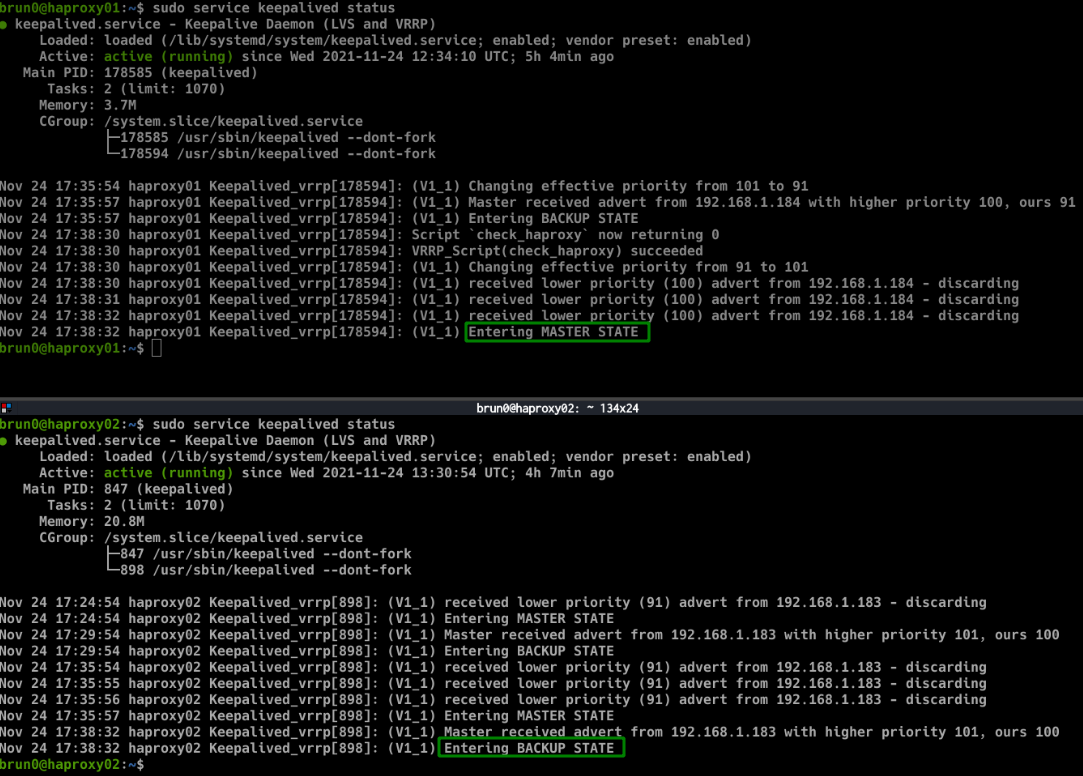
\includegraphics[width=14cm]{imagens/experiencias/02_terminal_haproxy_retomado.png}
\caption{Estado final do KeepAlived - Experiência 02}
\label{fig.nav}
\end{figure}

\subsubsection{Problemas encontrados na Experiência 02}
\paragraph{}
Com esta nova arquitetura, foi possível resolver um SPOF\textbf{(Single Point of Failure)} colocando mais um servidor de balanceamento de carga e acrescentando o serviço de \textbf{KeepAlived}, no entanto é notório que continua a existir um SPOF na base de dados.

\begin{figure}[H]
\center
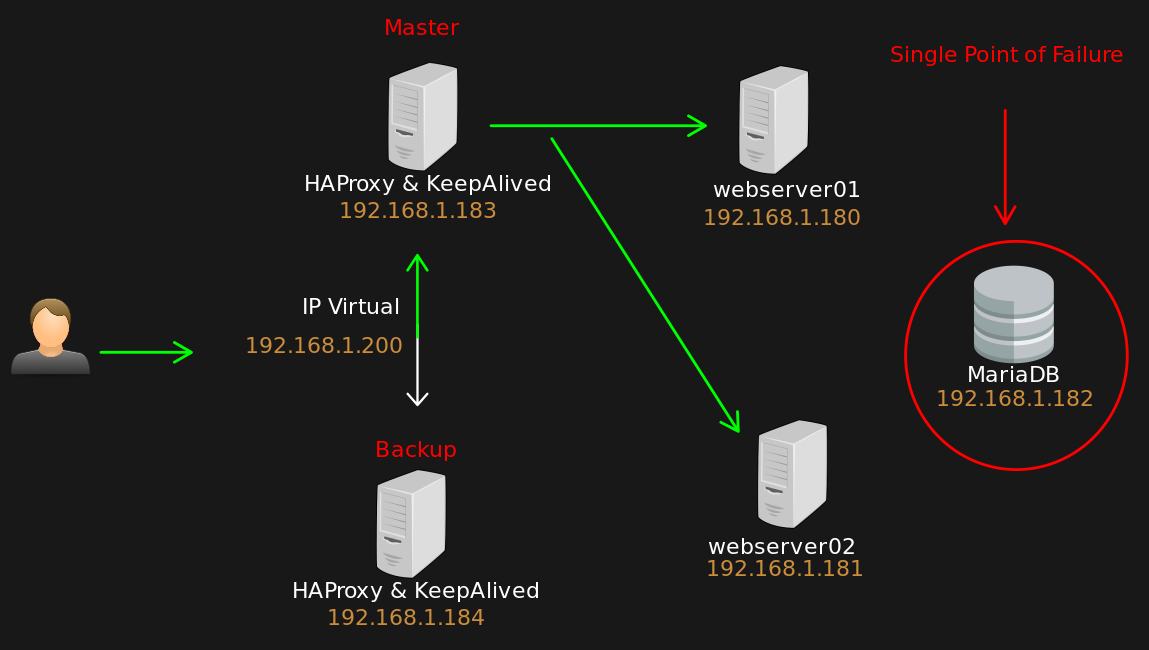
\includegraphics[width=12cm]{imagens/experiencias/02_spof.png}
\caption{Single Point of Failure - Experiência 02}
\label{fig.nav}
\end{figure}


\subsection{Experiência 03}
\paragraph{}
Para resolver o SPOF encontrado na última experiência, foi preciso utilizar mais um servidor HAProxy(\textbf{192.168.185}) e mais uma base de dados(\textbf{192.168.1.186}). Esta base de dados agora vai-se juntar à base de dados (\textbf{192.168.1.182}) já existente fazendo assim um \textbf{\emph{Galera Cluster}}.

\paragraph{}
No primeiro servidor de base de dados (\textbf{192.168.1.182}) foi criado o ficheiro \textbf{galera.cnf} localizado em \textbf{\emph{/etc/mysql/mariadb.conf.d/galera.cnf}} contendo todas as configurações necessárias para a configuração do \emph{cluster}.


\begin{figure}[H]
\center
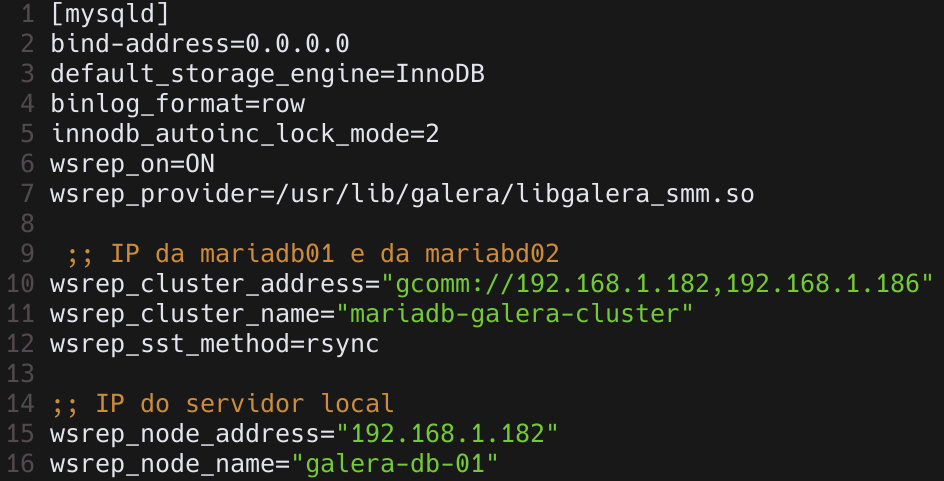
\includegraphics[width=12cm]{imagens/galeracluster_01.png}
\caption{Configuração do \emph{Galera Cluster} no mariadb01 - Experiência 03}
\label{fig.nav}
\end{figure}

\paragraph{}
No segundo servidor de base de dados (\textbf{192.168.1.186}) foi tambem criado o ficheiro \textbf{galera.cnf} com as configurações necessárias ao mesmo fazer parte do \emph{cluster}.

\begin{figure}[H]
\center
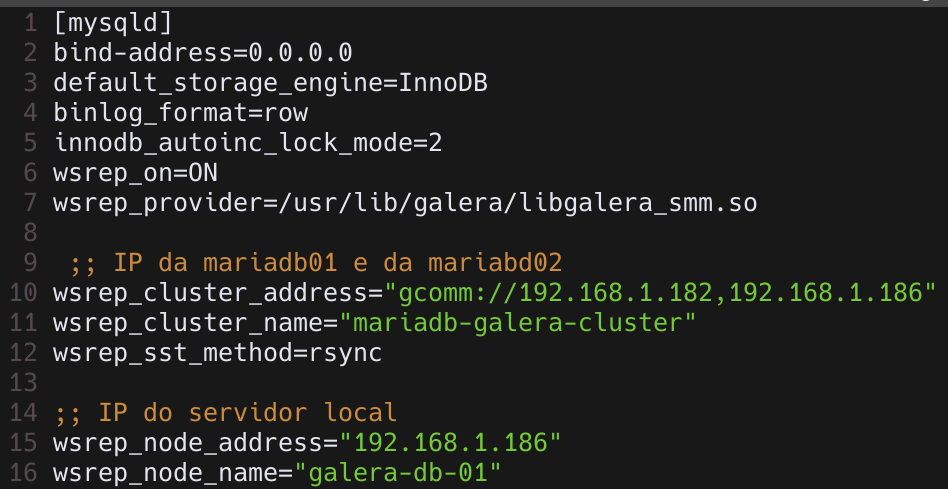
\includegraphics[width=12cm]{imagens/galeracluster_02.png}
\caption{Configuração do \emph{Galera Cluster} no mariadb02 - Experiência 03}
\label{fig.nav}
\end{figure}

\paragraph{}
Depois de ambos os servidores de base de dados configurados, foi visto que o tamanho do \emph{cluster} era de 2, para isso foi utilizado o comando \textbf{\emph{sudo mysql -u root -p -e "show status like 'wsrep\_cluster\_size'"}}.

\begin{figure}[H]
\center
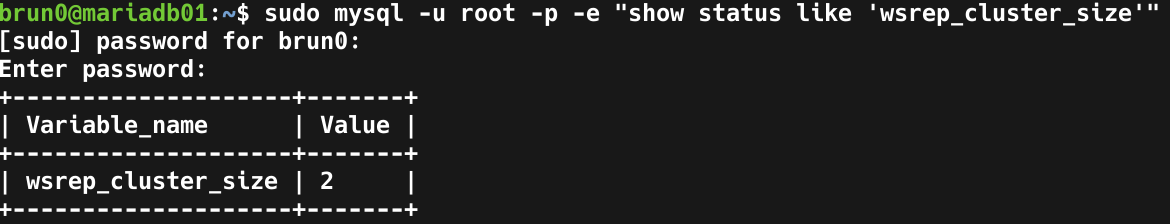
\includegraphics[width=12cm]{imagens/galeracluster_03.png}
\caption{Tamanho do \emph{Galera Cluster} - Experiência 03}
\label{fig.nav}
\end{figure}

\paragraph{}
De seguida o novo servidor de HAProxy (\textbf{192.168.1.185}) foi configurado de modo a receber e encaminhar tráfego dos clientes e das base de dados, fazendo assim um balanceamento de carga entre as bases de dados existentes no \emph{Galera Cluster}.\\
Para isto, foi editado o ficheiro \textbf{haproxy.cfg} localizado em \textbf{\emph{/etc/haproxy/haproxy.cfg}}.

\begin{figure}[H]
\center
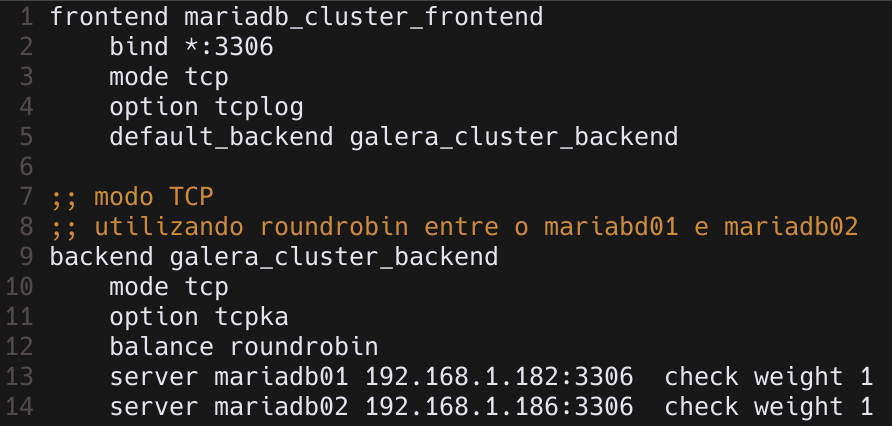
\includegraphics[width=12cm]{imagens/haproxy_config_03.png}
\caption{Configuração do HAProxy - Experiência 03}
\label{fig.nav}
\end{figure}

\paragraph{}
Por fim, foi necessário alterar o IP presente na variável de ambiente \textbf{DB\_HOST}, em ambos os \emph{webservers}, de \textbf{192.168.1.182} para o IP do HAProxy (\textbf{192.168.1.185}).

\begin{figure}[H]
\center
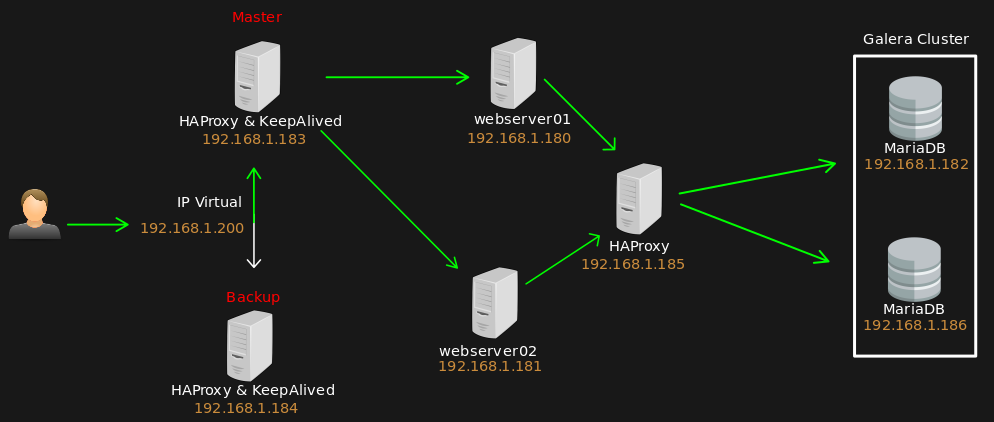
\includegraphics[width=14cm]{imagens/experiencias/03_1.png}
\caption{Esquema - Experiência 03}
\label{fig.nav}
\end{figure}
\clearpage
\subsubsection{Resultado}
\paragraph{}
Foi realizada uma captura no HAProxy03 (\textbf{192.168.1.185}) usando o \emph{wireshark} para perceber como é que o tráfego circulava na rede.\\

Inicialmente o \emph{webserver01} emite um \textbf{\emph{ARP Request}} para saber qual é o \textbf{MAC} do novo HAProxy (\textbf{192.168.1.185}), sendo que o HAProxy transmite o seu \textbf{MAC} e logo a seguir faz uma saudação (\emph{Server Greeting}) à base de dados que neste caso foi à mariadb01 (\textbf{192.168.1.182}).\\
De seguida existe um \emph{Login Request} e é percetivel que agora a comunicação entre \emph{webserver} e base de dados, passa sempre pelo HAProxy.

\begin{figure}[H]
\center
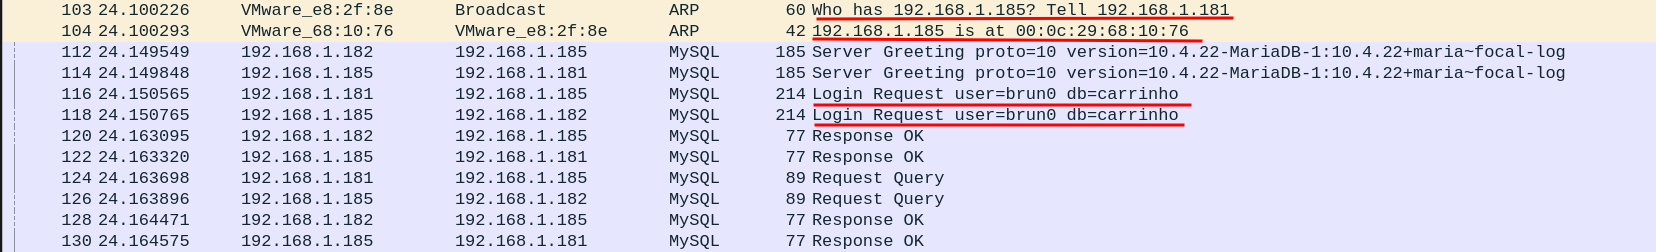
\includegraphics[width=16cm]{imagens/experiencias/03_primeira_conexao_e_query.png}
\caption{Primeira conexão - Experiência 03}
\label{fig.nav}
\end{figure}

\paragraph{}
Passado algum tempo, e já tendo sido feito o \emph{login} na aplicação, foi atualizada a página do \textbf{carrinho} e mais uma vez aqui é notório o caminho da comunicação entre \emph{webserver} e base de dados.\\
Desta vez o HAProxy encaminhou a \emph{query} do cliente para a mariadb02 (\textbf{192.168.1.186}) e posteriormente esta respondeu ao HAProxy voltando a ser encaminhada essa resposta para o cliente.

\begin{figure}[H]
\center
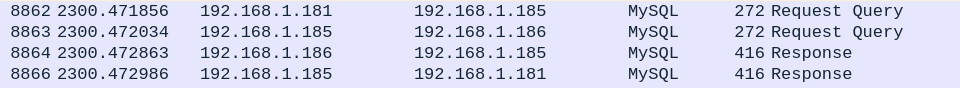
\includegraphics[width=15cm]{imagens/experiencias/03_atualizada_a_pagina.png}
\caption{Atualizada a página da aplicação - Experiência 03}
\label{fig.nav}
\end{figure}

\begin{figure}[H]
\center
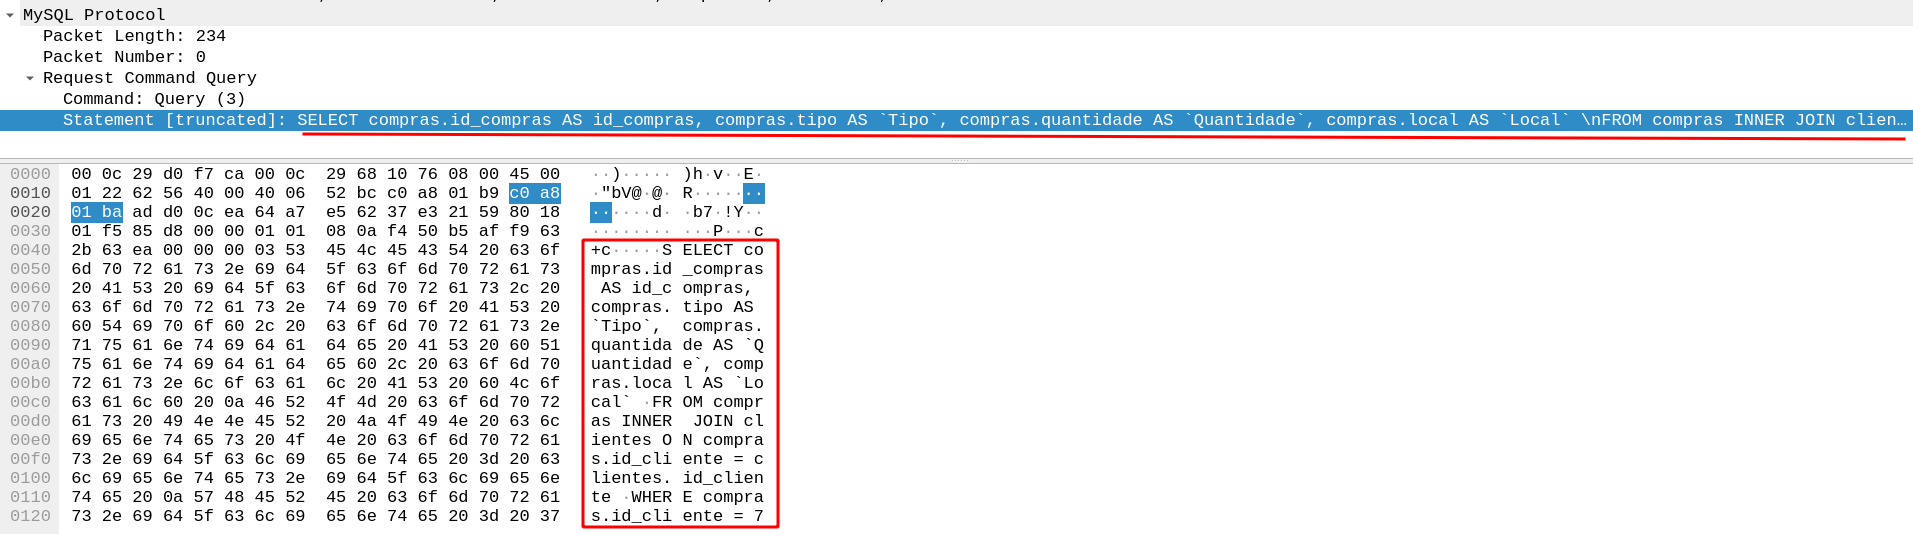
\includegraphics[width=16cm]{imagens/experiencias/03_atualizada_a_pagina_sql.png}
\caption{\emph{Query} SQL depois de atualizada a página da aplicação - Experiência 03}
\label{fig.nav}
\end{figure}


\subsubsection{Problemas encontrados na Experiência 03}
\paragraph{}
Com a implementação do novo HAProxy e do \emph{Galera Cluster}, foi possível resolver um SPOF que a antiga experiência tinha, no entanto passou a haver outro SPOF, agora no servidor de HAProxy que gere o \emph{Galera Cluster}. 

\begin{figure}[H]
\center
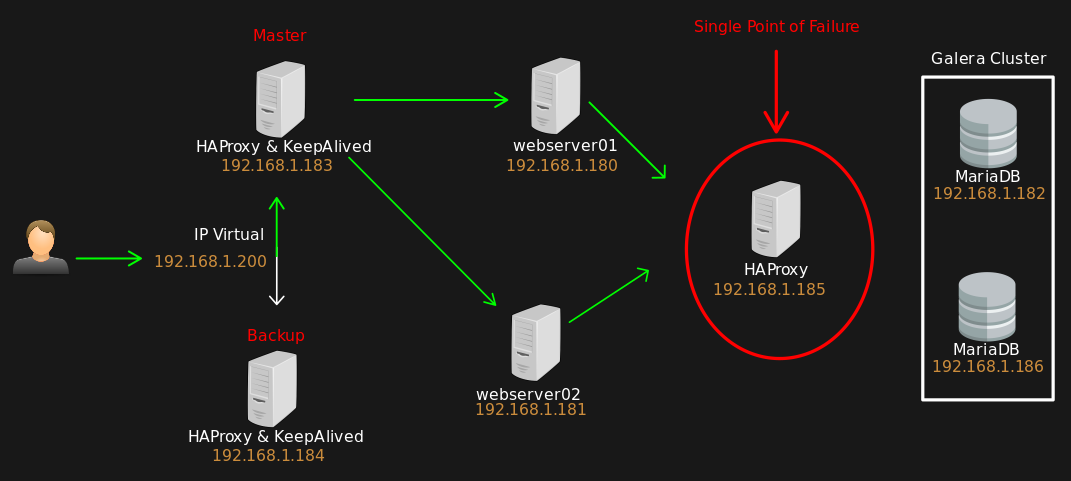
\includegraphics[width=16cm]{imagens/experiencias/03_spof.png}
\caption{Single Point of Failure - Experiência 03}
\label{fig.nav}
\end{figure}

\subsection{Experiência 04}
\paragraph{}
Para resolver o SPOF encontrado na última experiência, foi preciso utilizar mais um servidor de HAProxy (\textbf{192.168.1.187}) e acrescentar o KeepAlived em ambos os servidores HAProxy que fazem o balanceamento de carga para o \emph{Galera Cluster}.

\begin{figure}[H]
\center
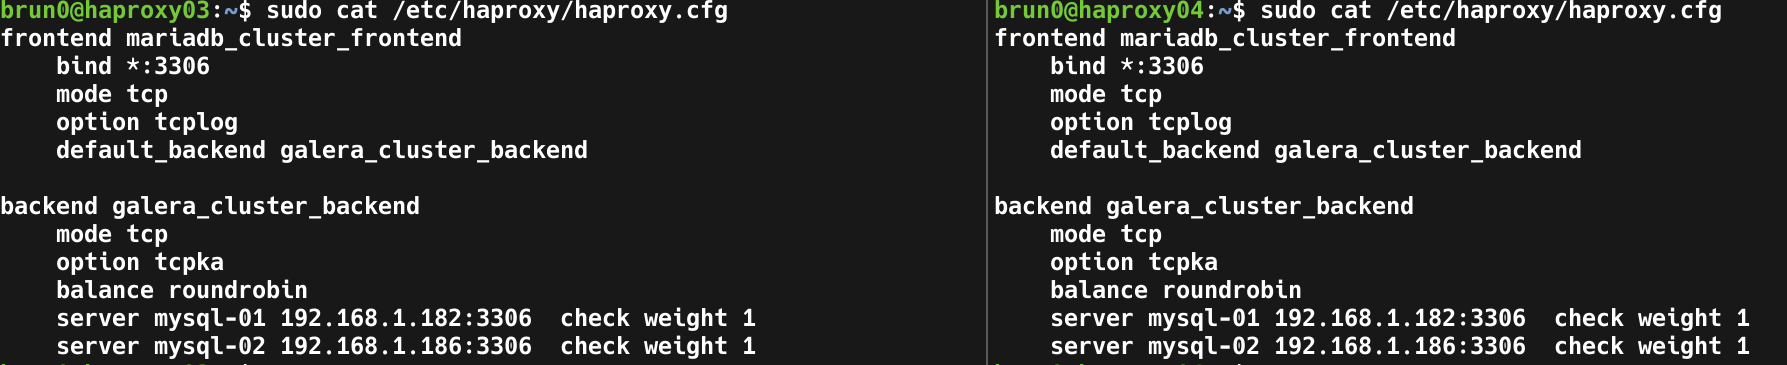
\includegraphics[width=14cm]{imagens/haproxy_04.png}
\caption{Configuração do HAProxy - Experiência 04}
\label{fig.nav}
\end{figure}


\paragraph{}
A configuração do KeepAlived foi exatamente igual, no entanto para estes dois servidores de HAProxy foi utilizado o ip virtual \textbf{192.168.1.250}, tendo na mesma um \textbf{\emph{vrrp\_script}} que faz o controlo da "vida" dos servidores de HAProxy.

\begin{figure}[H]
\center
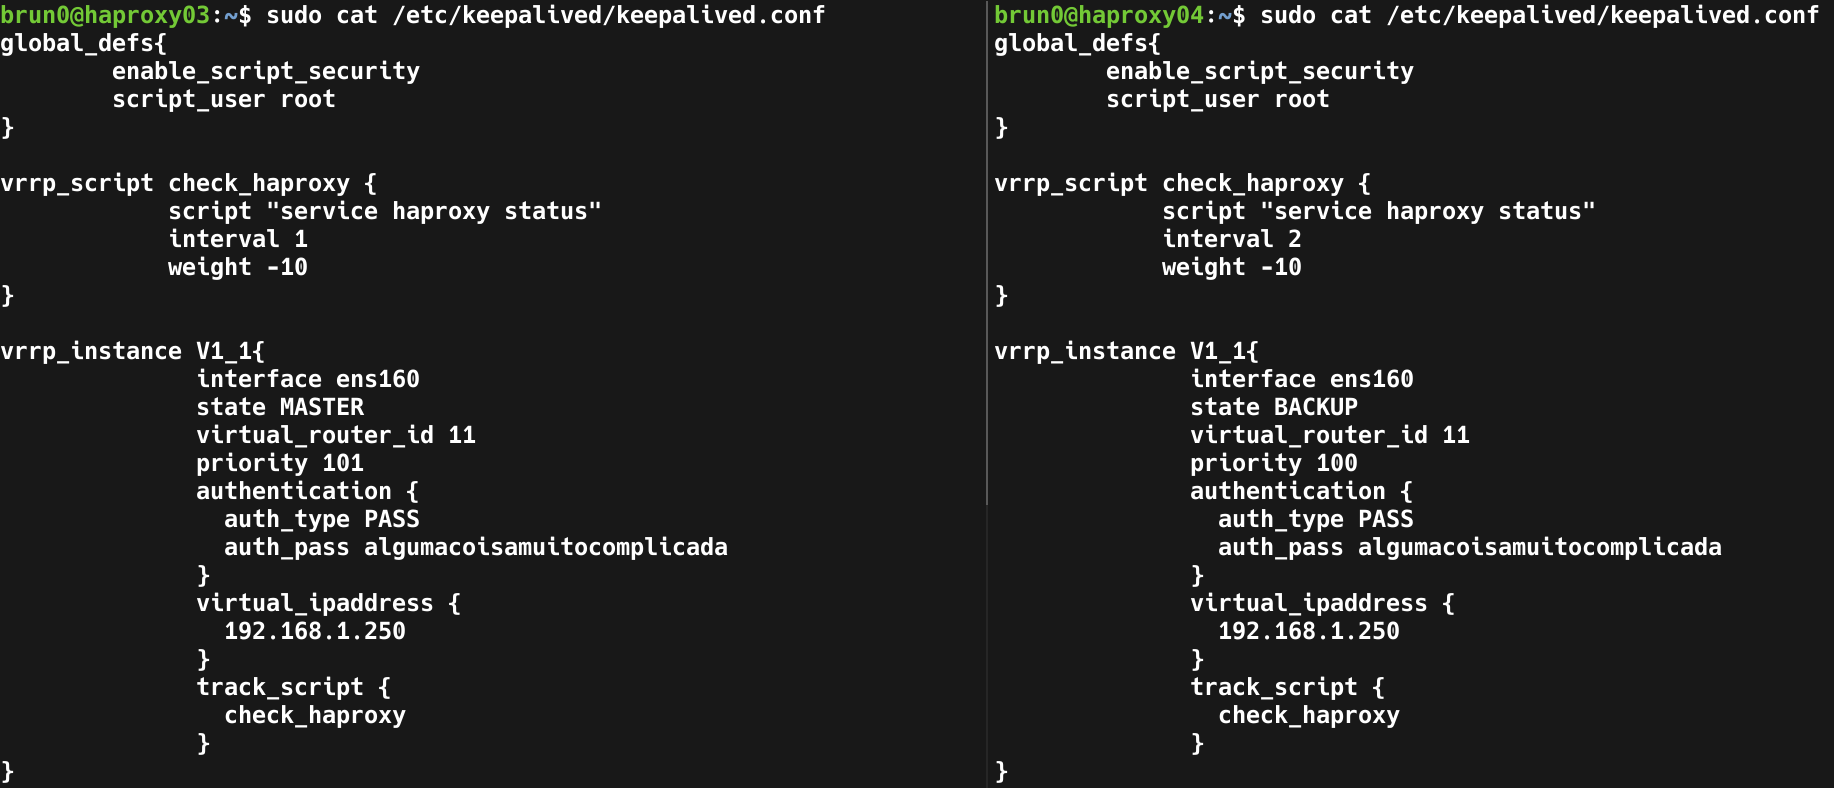
\includegraphics[width=13cm]{imagens/keepalived_04.png}
\caption{Configuração do KeepAlived - Experiência 04}
\label{fig.nav}
\end{figure}


\paragraph{}
Por fim, foi necessário alterar o IP presente na variável de ambiente \textbf{DB\_HOST}, em ambos os \emph{webservers},
de \textbf{192.168.1.185} (IP do HAProxy03) para o IP virtual (\textbf{192.168.1.185}).

\begin{figure}[H]
\center
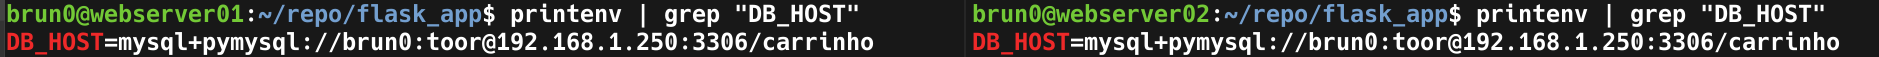
\includegraphics[width=17cm]{imagens/dbhost_04.png}
\caption{Variável de ambiente DB\_HOST - Experiência 04}
\label{fig.nav}
\end{figure}


\begin{figure}[H]
\center
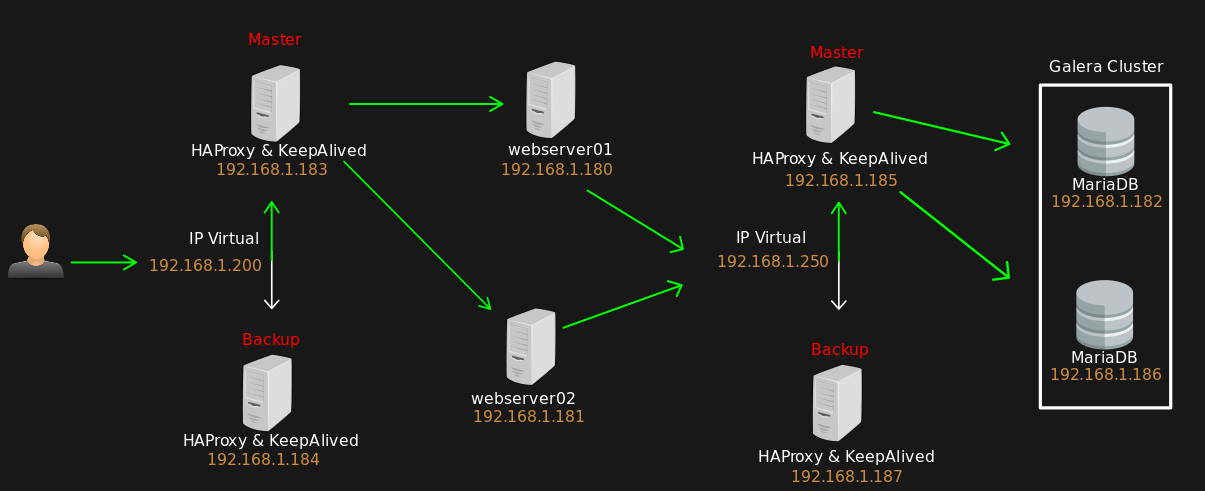
\includegraphics[width=16cm]{imagens/experiencias/04_1.png}
\caption{Esquema - Experiência 04}
\label{fig.nav}
\end{figure}

\begin{figure}[H]
\center
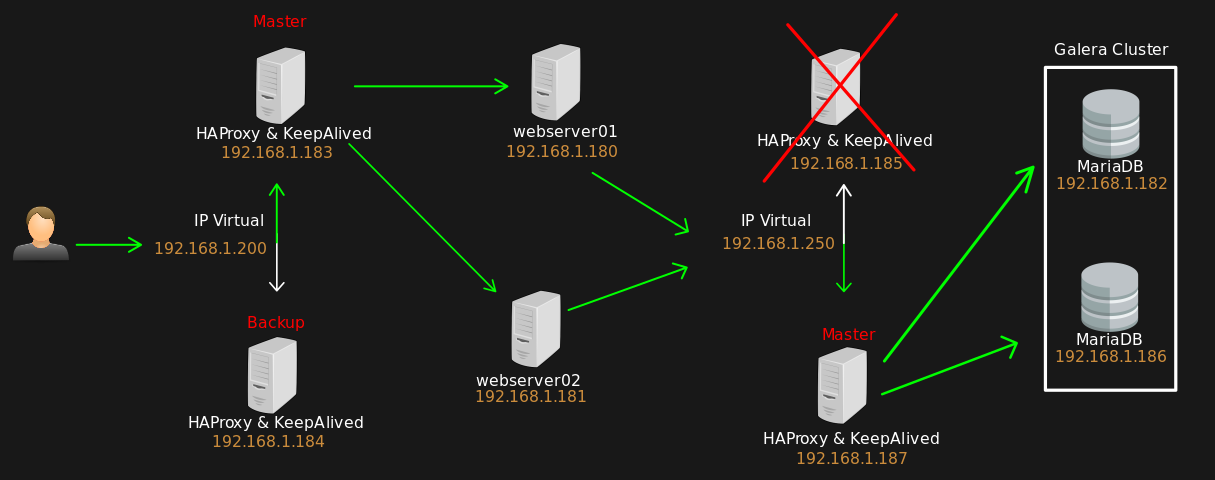
\includegraphics[width=16cm]{imagens/experiencias/04_2.png}
\caption{Esquema com \emph{failover} - Experiência 04}
\label{fig.nav}
\end{figure}


\subsubsection{Resultado}
\paragraph{}
Foram feitas capturas, tanto no \textbf{HAProxy03}(\textbf{MASTER}) como no \textbf{HAProxy04}(\textbf{BACKUP})
usando o \emph{wireshark}.\\
Como visto anteriormente, o HAProxy03(\textbf{192.168.1.185}) como é o \emph{MASTER}, envia, de segundo em segundo, um \emph{announcement} indicando a sua pioridade enquanto que o HAProxy04(\textbf{192.168.1.187}) está à escuta.
Na captura do \emph{wireshark} é possível tambem ver o \emph{announcement} vindo do HAProxy01(\textbf{192.168.1.183}).

\begin{figure}[H]
\center
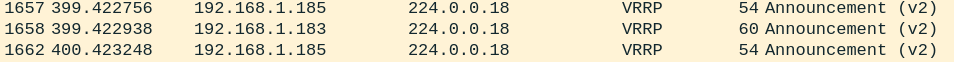
\includegraphics[width=16cm]{imagens/experiencias/04_wireshark_1.png}
\caption{\emph{Announcements} do HAProxy01 e HAProxy03 - Experiência 04}
\label{fig.nav}
\end{figure}

\paragraph{}
Depois de desligar o serviço HAProxy do HAProxy03(\textbf{192.168.1.185}), o mesmo fica com uma prioridade de 91 passando assim para o estado de \emph{BACKUP} ao mesmo tempo que o HAProxy04(\textbf{192.168.1.187}) passa para o estado de \emph{MASTER} uma vez que a sua prioridade é superior (100).

\begin{figure}[H]
\center
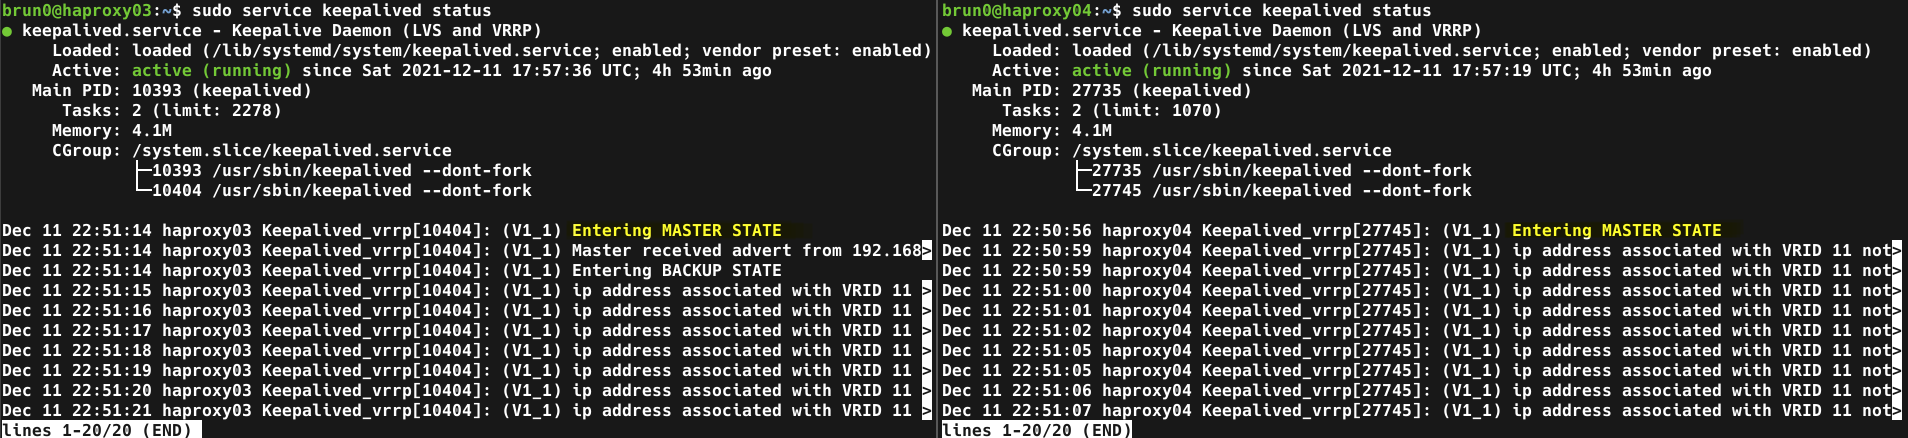
\includegraphics[width=16cm]{imagens/experiencias/04_desligado_haproxy03.png}
\caption{Troca de \emph{MASTER} e \emph{BACKUP} - Experiência 04}
\label{fig.nav}
\end{figure}

\paragraph{}
Neste momento continua a haver uma conexão normal do cliente para os \emph{webservers}, sendo que os mesmos continuam a conseguir fazer \emph{querys} às bases de dados como se nada tivesse acontecido.\\
Depois de ser reativado o serviço de HAProxy no HAProxy03, o mesmo passa novamente a ser \emph{MASTER} visto que a sua prioridade volta a aumentar.

\begin{figure}[H]
\center
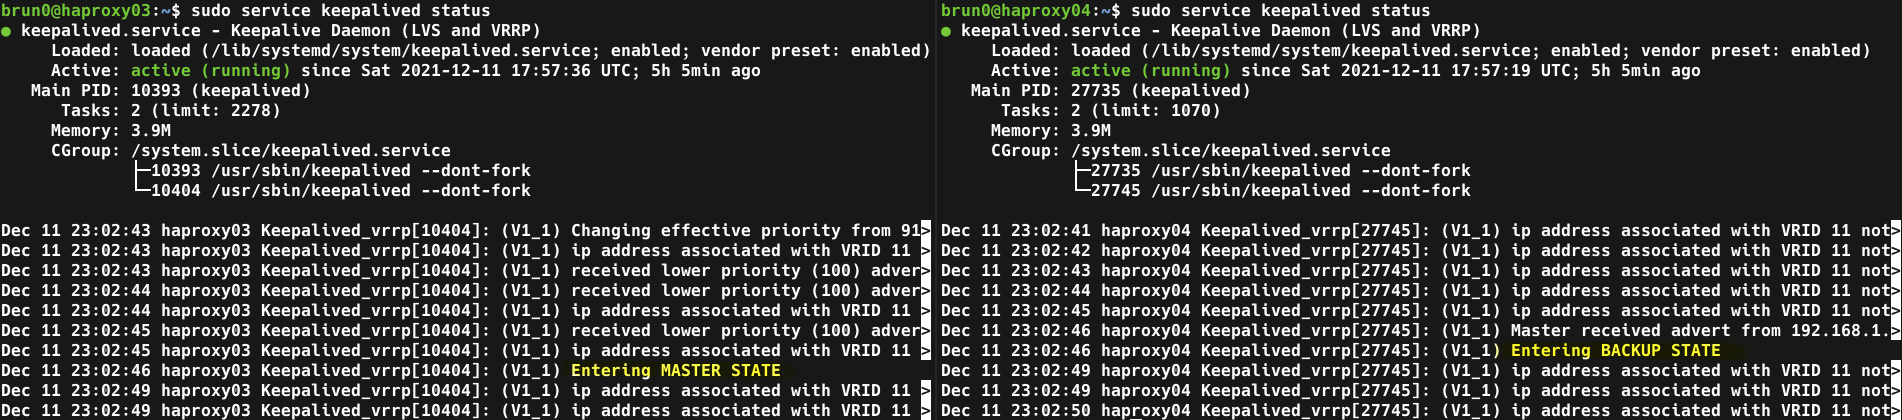
\includegraphics[width=16cm]{imagens/experiencias/04_reativado_haproxy03.png}
\caption{Reativado serviço HAProxy em HAProxy03 - Experiência 04}
\label{fig.nav}
\end{figure}

Por fim, podemos concluir que com esta arquitetura temos uma infraestrutura minimamente segura, capaz de ser disponível e de garantir desempenho. Tudo isto se deve aos vários \emph{proxies} implementados assim como o \emph{galera cluster} que oferece uma redundância enorme para um bom desempenho da infraestrutura.\\
A implementação final, não apresenta nenhum SPOF, cumprindo assim o objetivo proposto no inicio do trabalho.

\chapter{Conclusão}\label{Conclusão}
\paragraph{}
Com a execução destas experiências foi possível perceber a importância que tem a disponibilidade e o desempenho numa infraestrutura que fornece serviços \emph{web}. \\
Inicialmente existia um pequeno problema (\textbf{como resolver 2 SPOFs?}), porém com a resolução desses problemas, foram aparecendo outros que à primeira vista aparentavam ser pequenos, no entanto os mesmos prejudicavam a infraestrutura num todo, fazendo com que a mesma ficasse inoperacional.
\paragraph{}
A partir daqui foi percetível que antes de ser implementada e tornada operacional uma infraestrutura que fornece um serviço qualquer a mesma tem de ser bem planeada de modo a não ser preciso acrescentar muitos mais recursos aos inicialmente pensados.\\
Para isso é necessário criar um planeamento a pensar em todos os \emph{single point of failures} que possam existir e como os conseguimos resolver, tornando assim a infraestrutura disponível e ao mesmo tempo com um bom desempenho fazendo uso do balanceamento de carga.


\begin{acronym}
\acro{isec}[ISEC]{Instituto Superior de Engenharia de Coimbra}
\acro{deis}[DEIS]{Departamento de Engenharia Informática e de Sistemas}
\acro{lei}[LEI]{Licenciatura em Engenharia Informática}
\end{acronym}



\begin{thebibliography}{9}
\bibitem{stackov} 
Stack Overflow
\\\texttt{https://stackoverflow.com/}

\bibitem{mariadbgaleracluster}
Mariadb e Galera Cluster
\\\texttt{https://mariadb.com/kb/en/what-is-mariadb-galera-cluster/}

\bibitem{flask}
Flask
\\\texttt{https://flask.palletsprojects.com/en/2.0.x/}

\bibitem{haproxy}
HAProxy
\\\texttt{https://www.digitalocean.com/community/tutorials/an-introduction-to-haproxy-and-load\-balancing-concepts}

\bibitem{keepalived}
Keepalived
\\\texttt{https://www.redhat.com/sysadmin/keepalived-basics}

\end{thebibliography}


\end{document}
